\chapter{Main Processor Module} \label{sec:MCU}

This section outlines the behavior of the main processor, or MCU. The MCU processes sampled voltage and current waveforms and configures the Sample Control Module with parameters like sample size, sample frequency, and test frequency. Although the original plan was for the Sample Control Module to manage tasks such as auto-ranging, adjusting PGA gain, and setting the test-signal level, these have been incorporated into the MCU's responsibilities due to time constraints. Implementing such non-time-critical functions in C rather than HDL proved to be both easier and quicker.

The process for determining the impedance of a Device Under Test (DUT) involves several steps and can be seen on figure \refq{fig:7_x_MCULOOP}.

\begin{figure}[H]
    \centering
    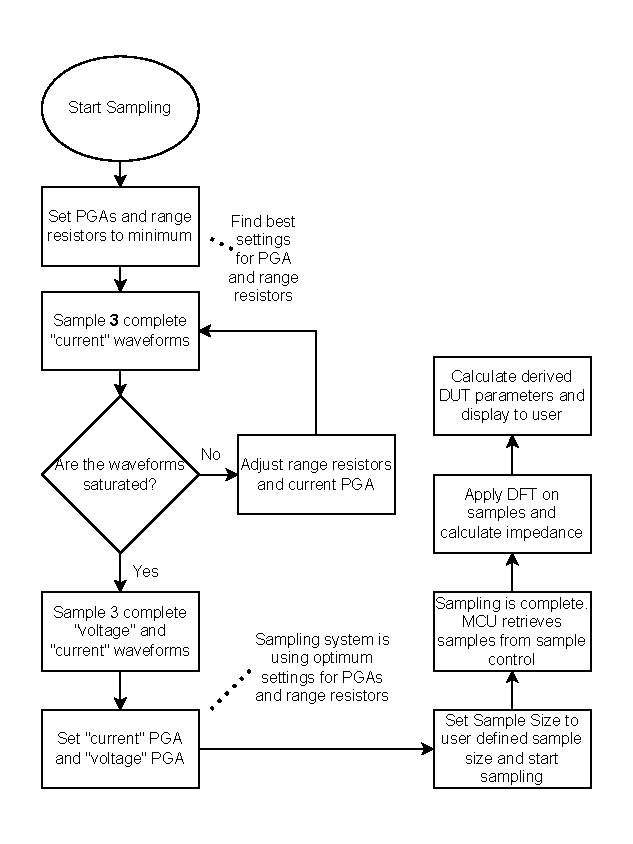
\includegraphics[clip, trim=0 15 15 0, width=0.60\textwidth]{Sections/7_SystemDesign/Figures/MainProcessorFunction.pdf}
    \caption{The figure shows a simplified flow chart for the MCU to start a sampling process, retrieving the samples and performing spectral analysis, in order to calculate the impedance of the DUT and the derived quantities.}
    \label{fig:7_x_MCULOOP}
\end{figure}

Initially, a small sample size, capturing just a few full waveforms of the test frequency, is set for the Sample Control Module as shown on figure \refq{fig:7_x_MCULOOP}. Sampling begins, and after completion, the MCU checks if the sampled signal is either saturated, or not fully utilizing the ADC's full dynamic range. Based on this check, adjustments are made to the range resistors and PGA settings. 

Next, the sample size is adjusted in the Sample Control Module, and sampling is reinitiated. Once the new sampling is done, the MCU retrieves these samples, applies a Discrete Fourier Transform (DFT) to analyze them, and then calculates the impedance using the frequency-domain representations of voltage and current. After calculation, necessary corrections are applied to the impedance values. The final step, which was not completed by the time of this report, involves displaying this impedance through a user interface.

The key segments of the C code executed on the STM32F446RE microcontroller are detailed in this section. The full C code can be found in appendix \refq{App:MCUCode}. The C code for the project makes use of ST's HAL (Hardware Abstraction Layer) drivers \cite{STHAL}, to access GPIO functions, UARTs and timers. These HAL drivers are generic callback functions and are common to the entire STM32 platform, which makes it possible to easily swap the STM32F446RE to a different microcontroller if, for whatever reason, more memory, more GPIO pins, more UARTs, timers or other hardware modules are required. The control registers for the microcontroller have, in some cases, also been manipulated directly in order to increase efficiency of the code as will be seen in this chapter. 




